\section{Dataset}
\label{sec:data}

This section describes the dataset we collected to facilitate our
experiments.  We collected our dataset as mappings between code and
natural language elements from large and popular evolving projects.
For our tasks, we extract methods (as code elements) and method names
and \javadoc comments as natural language elements.  In our study, we
chose to use only projects written in the Java programming language,
because \Fix{most/all} prior work focused on this language.  We also
focus only on comments that are written in English to be consistent
with prior work.  In the future, it would be worth studying other
programming and natural languages.

%The code is Java methods, and the natural language elements are the
%names and \javadoc comments of those methods.

We started with the \NumProjectPlanned Java projects on GitHub that
have the most stars (i.e., most number of users who liked the
projects).  This approach was used in \Fix{most} recent related work.
We then discarded the projects where no valid data could be collected
(e.g., no method \javadoc) or are obviously not software projects
(e.g.,
\href{https://github.com/CyC2018/CS-Notes}{CyC2018/CS-Notes}). After
this filtering, we ended up with \NumProject projects.  For each
project, we then performed the following steps:
\begin{enumerate}
\item clone the project;
\item checkout revisions on \ajanone{} of each year from 2017 to 2020;
\item at each revision, find all \CodeIn{*.java} files and use
  JavaParser~\cite{JavaParser} to parse the files;
\item collect all method bodies (removing inline comments from them)
  and their \javadoc, but discarding the data that matches any of the
  following conditions: (a) the method is abstract; (b) the \javadoc
  summary is empty; (c) the method body or the \javadoc summary
  contains non-English characters; (d) the method body is longer than
  10,000 characters.\Fix{how many for each}
\end{enumerate}

The final dataset consists of \NumDataAll unique method-\javadoc pairs
across all \NumRevisionAll revisions (\NumDataLatest from the latest
revision at \ajanone{}, 2020).

We implement the \filterfunc $F(d_1, d_2)$ to keep only the new
methods in $d_2$ that do not exist in $d_1$, by removing the method
that has the same tuple of class name, method name, and method
arguments:
\begin{flalign*}
  &F(d_1, d_2) = \{ m | m \in d_2 \land \lqall{m' \in d_1} \\
  &\qquad (\mathtt{ClassName}(m), \mathtt{Name}(m), \mathtt{Arguments}(m)) \neq \\
  &\qquad\qquad (\mathtt{ClassName}(m'), \mathtt{Name}(m'), \mathtt{Arguments}(m'))\}
\end{flalign*}

\input{tables/table-CG-dataset-metrics-main}

%% Automatically generated by pyutil.latex 

\begin{table}
\begin{small}
\begin{center}
\caption{\TCDatasetMetricsMainMN}
\begin{tabular}{ l@{\hspace{2pt}}|@{\hspace{2pt}}c@{\hspace{2pt}} | r r r}
\toprule
\multicolumn{2}{c|}{} & & & \\
\multicolumn{2}{c|}{\multirow{-2}{*}{\THDSStat}} & \multirow{-2}{*}{\UseMacro{TH-ds-all}} & \multirow{-2}{*}{\UseMacro{TH-ds-2020}} & \multirow{-2}{*}{\UseMacro{TH-ds-2019-2020}} \\
\midrule
\multicolumn{2}{c|}{\UseMacro{TH-ds-num-project}}
 & \UseMacro{ds-MN-num-proj}
 & \UseMacro{ds-MN-num-proj}
 & \UseMacro{ds-MN-num-proj}
\\
\multicolumn{2}{c|}{\UseMacro{TH-ds-num-data}}
 & \UseMacro{raw-ds-MN-num-data_all}
 & \UseMacro{ds-MN-num-data_2020}
 & \UseMacro{ds-MN-num-data_2019-2020}
\\
\midrule
& \UseMacro{TH-ds-len-method-avg}
 & \UseMacro{raw-ds-MN-len-meth-AVG_all}
 & \UseMacro{ds-MN-len-meth-AVG_2020}
 & \UseMacro{ds-MN-len-meth-AVG_2019-2020}
\\
& \UseMacro{TH-ds-len-method-mode}
 & \UseMacro{raw-ds-MN-len-meth-MODE_all}
 & \UseMacro{ds-MN-len-meth-MODE_2020}
 & \UseMacro{ds-MN-len-meth-MODE_2019-2020}
\\
& \UseMacro{TH-ds-len-method-median}
 & \UseMacro{raw-ds-MN-len-meth-MEDIAN_all}
 & \UseMacro{ds-MN-len-meth-MEDIAN_2020}
 & \UseMacro{ds-MN-len-meth-MEDIAN_2019-2020}
\\
& \UseMacro{TH-ds-len-method-le100}
 & \UseMacro{raw-ds-MN-len-meth-le-100_all}
 & \UseMacro{ds-MN-len-meth-le-100_2020}
 & \UseMacro{ds-MN-len-meth-le-100_2019-2020}
\\
& \UseMacro{TH-ds-len-method-le150}
 & \UseMacro{raw-ds-MN-len-meth-le-150_all}
 & \UseMacro{ds-MN-len-meth-le-150_2020}
 & \UseMacro{ds-MN-len-meth-le-150_2019-2020}
\\
\multirow{-6}{*}{\UseMacro{TH-ds-len-method}} & \UseMacro{TH-ds-len-method-le200}
 & \UseMacro{raw-ds-MN-len-meth-le-200_all}
 & \UseMacro{ds-MN-len-meth-le-200_2020}
 & \UseMacro{ds-MN-len-meth-le-200_2019-2020}
\\
\midrule
& \UseMacro{TH-ds-len-comment-avg}
 & \UseMacro{raw-ds-MN-len-com-AVG_all}
 & \UseMacro{ds-MN-len-com-AVG_2020}
 & \UseMacro{ds-MN-len-com-AVG_2019-2020}
\\
& \UseMacro{TH-ds-len-comment-mode}
 & \UseMacro{raw-ds-MN-len-com-MODE_all}
 & \UseMacro{ds-MN-len-com-MODE_2020}
 & \UseMacro{ds-MN-len-com-MODE_2019-2020}
\\
& \UseMacro{TH-ds-len-comment-median}
 & \UseMacro{raw-ds-MN-len-com-MEDIAN_all}
 & \UseMacro{ds-MN-len-com-MEDIAN_2020}
 & \UseMacro{ds-MN-len-com-MEDIAN_2019-2020}
\\
& \UseMacro{TH-ds-len-comment-le20}
 & \UseMacro{raw-ds-MN-len-com-le-20_all}
 & \UseMacro{ds-MN-len-com-le-20_2020}
 & \UseMacro{ds-MN-len-com-le-20_2019-2020}
\\
& \UseMacro{TH-ds-len-comment-le30}
 & \UseMacro{raw-ds-MN-len-com-le-30_all}
 & \UseMacro{ds-MN-len-com-le-30_2020}
 & \UseMacro{ds-MN-len-com-le-30_2019-2020}
\\
\multirow{-6}{*}{\UseMacro{TH-ds-len-comment}} & \UseMacro{TH-ds-len-comment-le50}
 & \UseMacro{raw-ds-MN-len-com-le-50_all}
 & \UseMacro{ds-MN-len-com-le-50_2020}
 & \UseMacro{ds-MN-len-com-le-50_2019-2020}
\\
\midrule
& \UseMacro{TH-ds-len-name-avg}
 & \UseMacro{raw-ds-MN-len-name-AVG_all}
 & \UseMacro{ds-MN-len-name-AVG_2020}
 & \UseMacro{ds-MN-len-name-AVG_2019-2020}
\\
& \UseMacro{TH-ds-len-name-mode}
 & \UseMacro{raw-ds-MN-len-name-MODE_all}
 & \UseMacro{ds-MN-len-name-MODE_2020}
 & \UseMacro{ds-MN-len-name-MODE_2019-2020}
\\
& \UseMacro{TH-ds-len-name-median}
 & \UseMacro{raw-ds-MN-len-name-MEDIAN_all}
 & \UseMacro{ds-MN-len-name-MEDIAN_2020}
 & \UseMacro{ds-MN-len-name-MEDIAN_2019-2020}
\\
& \UseMacro{TH-ds-len-name-le2}
 & \UseMacro{raw-ds-MN-len-name-le-3_all}
 & \UseMacro{ds-MN-len-name-le-3_2020}
 & \UseMacro{ds-MN-len-name-le-3_2019-2020}
\\
& \UseMacro{TH-ds-len-name-le3}
 & \UseMacro{raw-ds-MN-len-name-le-5_all}
 & \UseMacro{ds-MN-len-name-le-5_2020}
 & \UseMacro{ds-MN-len-name-le-5_2019-2020}
\\
\multirow{-6}{*}{\UseMacro{TH-ds-len-name}} & \UseMacro{TH-ds-len-name-le6}
 & \UseMacro{raw-ds-MN-len-name-le-6_all}
 & \UseMacro{ds-MN-len-name-le-6_2020}
 & \UseMacro{ds-MN-len-name-le-6_2019-2020}
\\
\bottomrule
\end{tabular}
\end{center}
\end{small}
\vspace{\TVDatasetMetricsMainMN}
\end{table}

\input{tables/table-CG-dataset-metrics-split}

%% Automatically generated by pyutil.latex 

\begin{table*}
\begin{small}
\begin{center}
\caption{\TCDatasetMetricsSplitMN}
\begin{tabular}{ l@{\hspace{2pt}}|@{\hspace{2pt}}c@{\hspace{2pt}} | rr @{\hspace{5pt}}c@{\hspace{5pt}} rr @{\hspace{5pt}}c@{\hspace{5pt}} rr r}
\toprule
\multicolumn{2}{c|}{} & \multicolumn{2}{c}{\UseMacro{TH-ds-mixedproj}} & & \multicolumn{2}{c}{\UseMacro{TH-ds-crossproj}} & & \multicolumn{2}{c}{\UseMacro{TH-ds-evo}} & \\\cline{3-4}\cline{6-7}\cline{9-10}
\multicolumn{2}{c|}{\multirow{-2}{*}{\THDSStat}} & \UseMacro{TH-ds-mixedproj-train} & \UseMacro{TH-ds-mixedproj-val} & & \UseMacro{TH-ds-crossproj-train} & \UseMacro{TH-ds-crossproj-val} & & \UseMacro{TH-ds-evo-train} & \UseMacro{TH-ds-evo-val} & \multirow{-2}{*}{\UseMacro{TH-ds-test}} \\
\midrule
\multicolumn{2}{c|}{\UseMacro{TH-ds-num-project}}
 & \UseMacro{ds-MN-num-proj}
 & \UseMacro{ds-MN-num-proj}
 & 
 & \UseMacro{ds-MN-num-proj_train}
 & \UseMacro{ds-MN-num-proj_val}
 & 
 & \UseMacro{ds-MN-num-proj}
 & \UseMacro{ds-MN-num-proj}
 & \UseMacro{ds-MN-num-proj_test}
\\
\multicolumn{2}{c|}{\UseMacro{TH-ds-num-data}}
 & \UseMacro{ds-MN-num-data_mixedproj-2020-train}
 & \UseMacro{ds-MN-num-data_mixedproj-2020-val}
 & 
 & \UseMacro{ds-MN-num-data_crossproj-2020-train}
 & \UseMacro{ds-MN-num-data_crossproj-2020-val}
 & 
 & \UseMacro{ds-MN-num-data_evo-2020-train}
 & \UseMacro{ds-MN-num-data_evo-2020-val}
 & \UseMacro{ds-MN-num-data_2020-test_common}
\\
\midrule
& \UseMacro{TH-ds-len-method-avg}
 & \UseMacro{ds-MN-len-meth-AVG_mixedproj-2020-train}
 & \UseMacro{ds-MN-len-meth-AVG_mixedproj-2020-val}
 & 
 & \UseMacro{ds-MN-len-meth-AVG_crossproj-2020-train}
 & \UseMacro{ds-MN-len-meth-AVG_crossproj-2020-val}
 & 
 & \UseMacro{ds-MN-len-meth-AVG_evo-2020-train}
 & \UseMacro{ds-MN-len-meth-AVG_evo-2020-val}
 & \UseMacro{ds-MN-len-meth-AVG_2020-test_common}
\\
& \UseMacro{TH-ds-len-method-mode}
 & \UseMacro{ds-MN-len-meth-MODE_mixedproj-2020-train}
 & \UseMacro{ds-MN-len-meth-MODE_mixedproj-2020-val}
 & 
 & \UseMacro{ds-MN-len-meth-MODE_crossproj-2020-train}
 & \UseMacro{ds-MN-len-meth-MODE_crossproj-2020-val}
 & 
 & \UseMacro{ds-MN-len-meth-MODE_evo-2020-train}
 & \UseMacro{ds-MN-len-meth-MODE_evo-2020-val}
 & \UseMacro{ds-MN-len-meth-MODE_2020-test_common}
\\
& \UseMacro{TH-ds-len-method-median}
 & \UseMacro{ds-MN-len-meth-MEDIAN_mixedproj-2020-train}
 & \UseMacro{ds-MN-len-meth-MEDIAN_mixedproj-2020-val}
 & 
 & \UseMacro{ds-MN-len-meth-MEDIAN_crossproj-2020-train}
 & \UseMacro{ds-MN-len-meth-MEDIAN_crossproj-2020-val}
 & 
 & \UseMacro{ds-MN-len-meth-MEDIAN_evo-2020-train}
 & \UseMacro{ds-MN-len-meth-MEDIAN_evo-2020-val}
 & \UseMacro{ds-MN-len-meth-MEDIAN_2020-test_common}
\\
& \UseMacro{TH-ds-len-method-le100}
 & \UseMacro{ds-MN-len-meth-le-100_mixedproj-2020-train}
 & \UseMacro{ds-MN-len-meth-le-100_mixedproj-2020-val}
 & 
 & \UseMacro{ds-MN-len-meth-le-100_crossproj-2020-train}
 & \UseMacro{ds-MN-len-meth-le-100_crossproj-2020-val}
 & 
 & \UseMacro{ds-MN-len-meth-le-100_evo-2020-train}
 & \UseMacro{ds-MN-len-meth-le-100_evo-2020-val}
 & \UseMacro{ds-MN-len-meth-le-100_2020-test_common}
\\
& \UseMacro{TH-ds-len-method-le150}
 & \UseMacro{ds-MN-len-meth-le-150_mixedproj-2020-train}
 & \UseMacro{ds-MN-len-meth-le-150_mixedproj-2020-val}
 & 
 & \UseMacro{ds-MN-len-meth-le-150_crossproj-2020-train}
 & \UseMacro{ds-MN-len-meth-le-150_crossproj-2020-val}
 & 
 & \UseMacro{ds-MN-len-meth-le-150_evo-2020-train}
 & \UseMacro{ds-MN-len-meth-le-150_evo-2020-val}
 & \UseMacro{ds-MN-len-meth-le-150_2020-test_common}
\\
\multirow{-6}{*}{\UseMacro{TH-ds-len-method}} & \UseMacro{TH-ds-len-method-le200}
 & \UseMacro{ds-MN-len-meth-le-200_mixedproj-2020-train}
 & \UseMacro{ds-MN-len-meth-le-200_mixedproj-2020-val}
 & 
 & \UseMacro{ds-MN-len-meth-le-200_crossproj-2020-train}
 & \UseMacro{ds-MN-len-meth-le-200_crossproj-2020-val}
 & 
 & \UseMacro{ds-MN-len-meth-le-200_evo-2020-train}
 & \UseMacro{ds-MN-len-meth-le-200_evo-2020-val}
 & \UseMacro{ds-MN-len-meth-le-200_2020-test_common}
\\
\midrule
& \UseMacro{TH-ds-len-comment-avg}
 & \UseMacro{ds-MN-len-com-AVG_mixedproj-2020-train}
 & \UseMacro{ds-MN-len-com-AVG_mixedproj-2020-val}
 & 
 & \UseMacro{ds-MN-len-com-AVG_crossproj-2020-train}
 & \UseMacro{ds-MN-len-com-AVG_crossproj-2020-val}
 & 
 & \UseMacro{ds-MN-len-com-AVG_evo-2020-train}
 & \UseMacro{ds-MN-len-com-AVG_evo-2020-val}
 & \UseMacro{ds-MN-len-com-AVG_2020-test_common}
\\
& \UseMacro{TH-ds-len-comment-mode}
 & \UseMacro{ds-MN-len-com-MODE_mixedproj-2020-train}
 & \UseMacro{ds-MN-len-com-MODE_mixedproj-2020-val}
 & 
 & \UseMacro{ds-MN-len-com-MODE_crossproj-2020-train}
 & \UseMacro{ds-MN-len-com-MODE_crossproj-2020-val}
 & 
 & \UseMacro{ds-MN-len-com-MODE_evo-2020-train}
 & \UseMacro{ds-MN-len-com-MODE_evo-2020-val}
 & \UseMacro{ds-MN-len-com-MODE_2020-test_common}
\\
& \UseMacro{TH-ds-len-comment-median}
 & \UseMacro{ds-MN-len-com-MEDIAN_mixedproj-2020-train}
 & \UseMacro{ds-MN-len-com-MEDIAN_mixedproj-2020-val}
 & 
 & \UseMacro{ds-MN-len-com-MEDIAN_crossproj-2020-train}
 & \UseMacro{ds-MN-len-com-MEDIAN_crossproj-2020-val}
 & 
 & \UseMacro{ds-MN-len-com-MEDIAN_evo-2020-train}
 & \UseMacro{ds-MN-len-com-MEDIAN_evo-2020-val}
 & \UseMacro{ds-MN-len-com-MEDIAN_2020-test_common}
\\
& \UseMacro{TH-ds-len-comment-le20}
 & \UseMacro{ds-MN-len-com-le-20_mixedproj-2020-train}
 & \UseMacro{ds-MN-len-com-le-20_mixedproj-2020-val}
 & 
 & \UseMacro{ds-MN-len-com-le-20_crossproj-2020-train}
 & \UseMacro{ds-MN-len-com-le-20_crossproj-2020-val}
 & 
 & \UseMacro{ds-MN-len-com-le-20_evo-2020-train}
 & \UseMacro{ds-MN-len-com-le-20_evo-2020-val}
 & \UseMacro{ds-MN-len-com-le-20_2020-test_common}
\\
& \UseMacro{TH-ds-len-comment-le30}
 & \UseMacro{ds-MN-len-com-le-30_mixedproj-2020-train}
 & \UseMacro{ds-MN-len-com-le-30_mixedproj-2020-val}
 & 
 & \UseMacro{ds-MN-len-com-le-30_crossproj-2020-train}
 & \UseMacro{ds-MN-len-com-le-30_crossproj-2020-val}
 & 
 & \UseMacro{ds-MN-len-com-le-30_evo-2020-train}
 & \UseMacro{ds-MN-len-com-le-30_evo-2020-val}
 & \UseMacro{ds-MN-len-com-le-30_2020-test_common}
\\
\multirow{-6}{*}{\UseMacro{TH-ds-len-comment}} & \UseMacro{TH-ds-len-comment-le50}
 & \UseMacro{ds-MN-len-com-le-50_mixedproj-2020-train}
 & \UseMacro{ds-MN-len-com-le-50_mixedproj-2020-val}
 & 
 & \UseMacro{ds-MN-len-com-le-50_crossproj-2020-train}
 & \UseMacro{ds-MN-len-com-le-50_crossproj-2020-val}
 & 
 & \UseMacro{ds-MN-len-com-le-50_evo-2020-train}
 & \UseMacro{ds-MN-len-com-le-50_evo-2020-val}
 & \UseMacro{ds-MN-len-com-le-50_2020-test_common}
\\
\midrule
& \UseMacro{TH-ds-len-name-avg}
 & \UseMacro{ds-MN-len-name-AVG_mixedproj-2020-train}
 & \UseMacro{ds-MN-len-name-AVG_mixedproj-2020-val}
 & 
 & \UseMacro{ds-MN-len-name-AVG_crossproj-2020-train}
 & \UseMacro{ds-MN-len-name-AVG_crossproj-2020-val}
 & 
 & \UseMacro{ds-MN-len-name-AVG_evo-2020-train}
 & \UseMacro{ds-MN-len-name-AVG_evo-2020-val}
 & \UseMacro{ds-MN-len-name-AVG_2020-test_common}
\\
& \UseMacro{TH-ds-len-name-mode}
 & \UseMacro{ds-MN-len-name-MODE_mixedproj-2020-train}
 & \UseMacro{ds-MN-len-name-MODE_mixedproj-2020-val}
 & 
 & \UseMacro{ds-MN-len-name-MODE_crossproj-2020-train}
 & \UseMacro{ds-MN-len-name-MODE_crossproj-2020-val}
 & 
 & \UseMacro{ds-MN-len-name-MODE_evo-2020-train}
 & \UseMacro{ds-MN-len-name-MODE_evo-2020-val}
 & \UseMacro{ds-MN-len-name-MODE_2020-test_common}
\\
& \UseMacro{TH-ds-len-name-median}
 & \UseMacro{ds-MN-len-name-MEDIAN_mixedproj-2020-train}
 & \UseMacro{ds-MN-len-name-MEDIAN_mixedproj-2020-val}
 & 
 & \UseMacro{ds-MN-len-name-MEDIAN_crossproj-2020-train}
 & \UseMacro{ds-MN-len-name-MEDIAN_crossproj-2020-val}
 & 
 & \UseMacro{ds-MN-len-name-MEDIAN_evo-2020-train}
 & \UseMacro{ds-MN-len-name-MEDIAN_evo-2020-val}
 & \UseMacro{ds-MN-len-name-MEDIAN_2020-test_common}
\\
& \UseMacro{TH-ds-len-name-le2}
 & \UseMacro{ds-MN-len-name-le-3_mixedproj-2020-train}
 & \UseMacro{ds-MN-len-name-le-3_mixedproj-2020-val}
 & 
 & \UseMacro{ds-MN-len-name-le-3_crossproj-2020-train}
 & \UseMacro{ds-MN-len-name-le-3_crossproj-2020-val}
 & 
 & \UseMacro{ds-MN-len-name-le-3_evo-2020-train}
 & \UseMacro{ds-MN-len-name-le-3_evo-2020-val}
 & \UseMacro{ds-MN-len-name-le-3_2020-test_common}
\\
& \UseMacro{TH-ds-len-name-le3}
 & \UseMacro{ds-MN-len-name-le-5_mixedproj-2020-train}
 & \UseMacro{ds-MN-len-name-le-5_mixedproj-2020-val}
 & 
 & \UseMacro{ds-MN-len-name-le-5_crossproj-2020-train}
 & \UseMacro{ds-MN-len-name-le-5_crossproj-2020-val}
 & 
 & \UseMacro{ds-MN-len-name-le-5_evo-2020-train}
 & \UseMacro{ds-MN-len-name-le-5_evo-2020-val}
 & \UseMacro{ds-MN-len-name-le-5_2020-test_common}
\\
\multirow{-6}{*}{\UseMacro{TH-ds-len-name}} & \UseMacro{TH-ds-len-name-le6}
 & \UseMacro{ds-MN-len-name-le-6_mixedproj-2020-train}
 & \UseMacro{ds-MN-len-name-le-6_mixedproj-2020-val}
 & 
 & \UseMacro{ds-MN-len-name-le-6_crossproj-2020-train}
 & \UseMacro{ds-MN-len-name-le-6_crossproj-2020-val}
 & 
 & \UseMacro{ds-MN-len-name-le-6_evo-2020-train}
 & \UseMacro{ds-MN-len-name-le-6_evo-2020-val}
 & \UseMacro{ds-MN-len-name-le-6_2020-test_common}
\\
\bottomrule
\end{tabular}
\end{center}
\end{small}
\vspace{\TVDatasetMetricsSplitMN}
\end{table*}


Table~\ref{table:dataset-metrics-main} and
Table~\ref{table:dataset-metrics-split} shows the statistics of
various parts of the dataset.
%
The statistics include (from the top row to the bottom row): number of
projects\Fix{same?}, number of methods, the \{average, mode, median\}
length (number of tokens) of method bodies, the percentage of methods
whose bodies length $\le$ \{100, 150, 200\}, the \{average, mode,
median\} length (number of tokens) of comments, the percentage of
methods whose comments length $\le$ \{20, 30, 50\}, the \{average,
mode, median\} length (number of sub-tokens) of method names, the
percentage of methods whose names length $\le$ \{2, 3, 6\}.
Table~\ref{table:dataset-metrics-main} lists the statistics for the
entire dataset, data available at 2020 ($\mathcal{D}(\mathcal{P},
2020)$), and new data between 2019 and 2020 ($\mathcal{D}(\mathcal{P},
2019, 2020)$); and Table~\ref{table:dataset-metrics-split} lists the
statistics for the \{\train, \val{}\} sets for the \mixedproj
\methodology, the \{\train, \val{}\} sets for the \crossproj
\methodology, the \{\train, \val{}\} sets for the \evoaware
\methodology, and the \test set which is common to all \methodologies.

\begin{figure}[t]
  \centering
  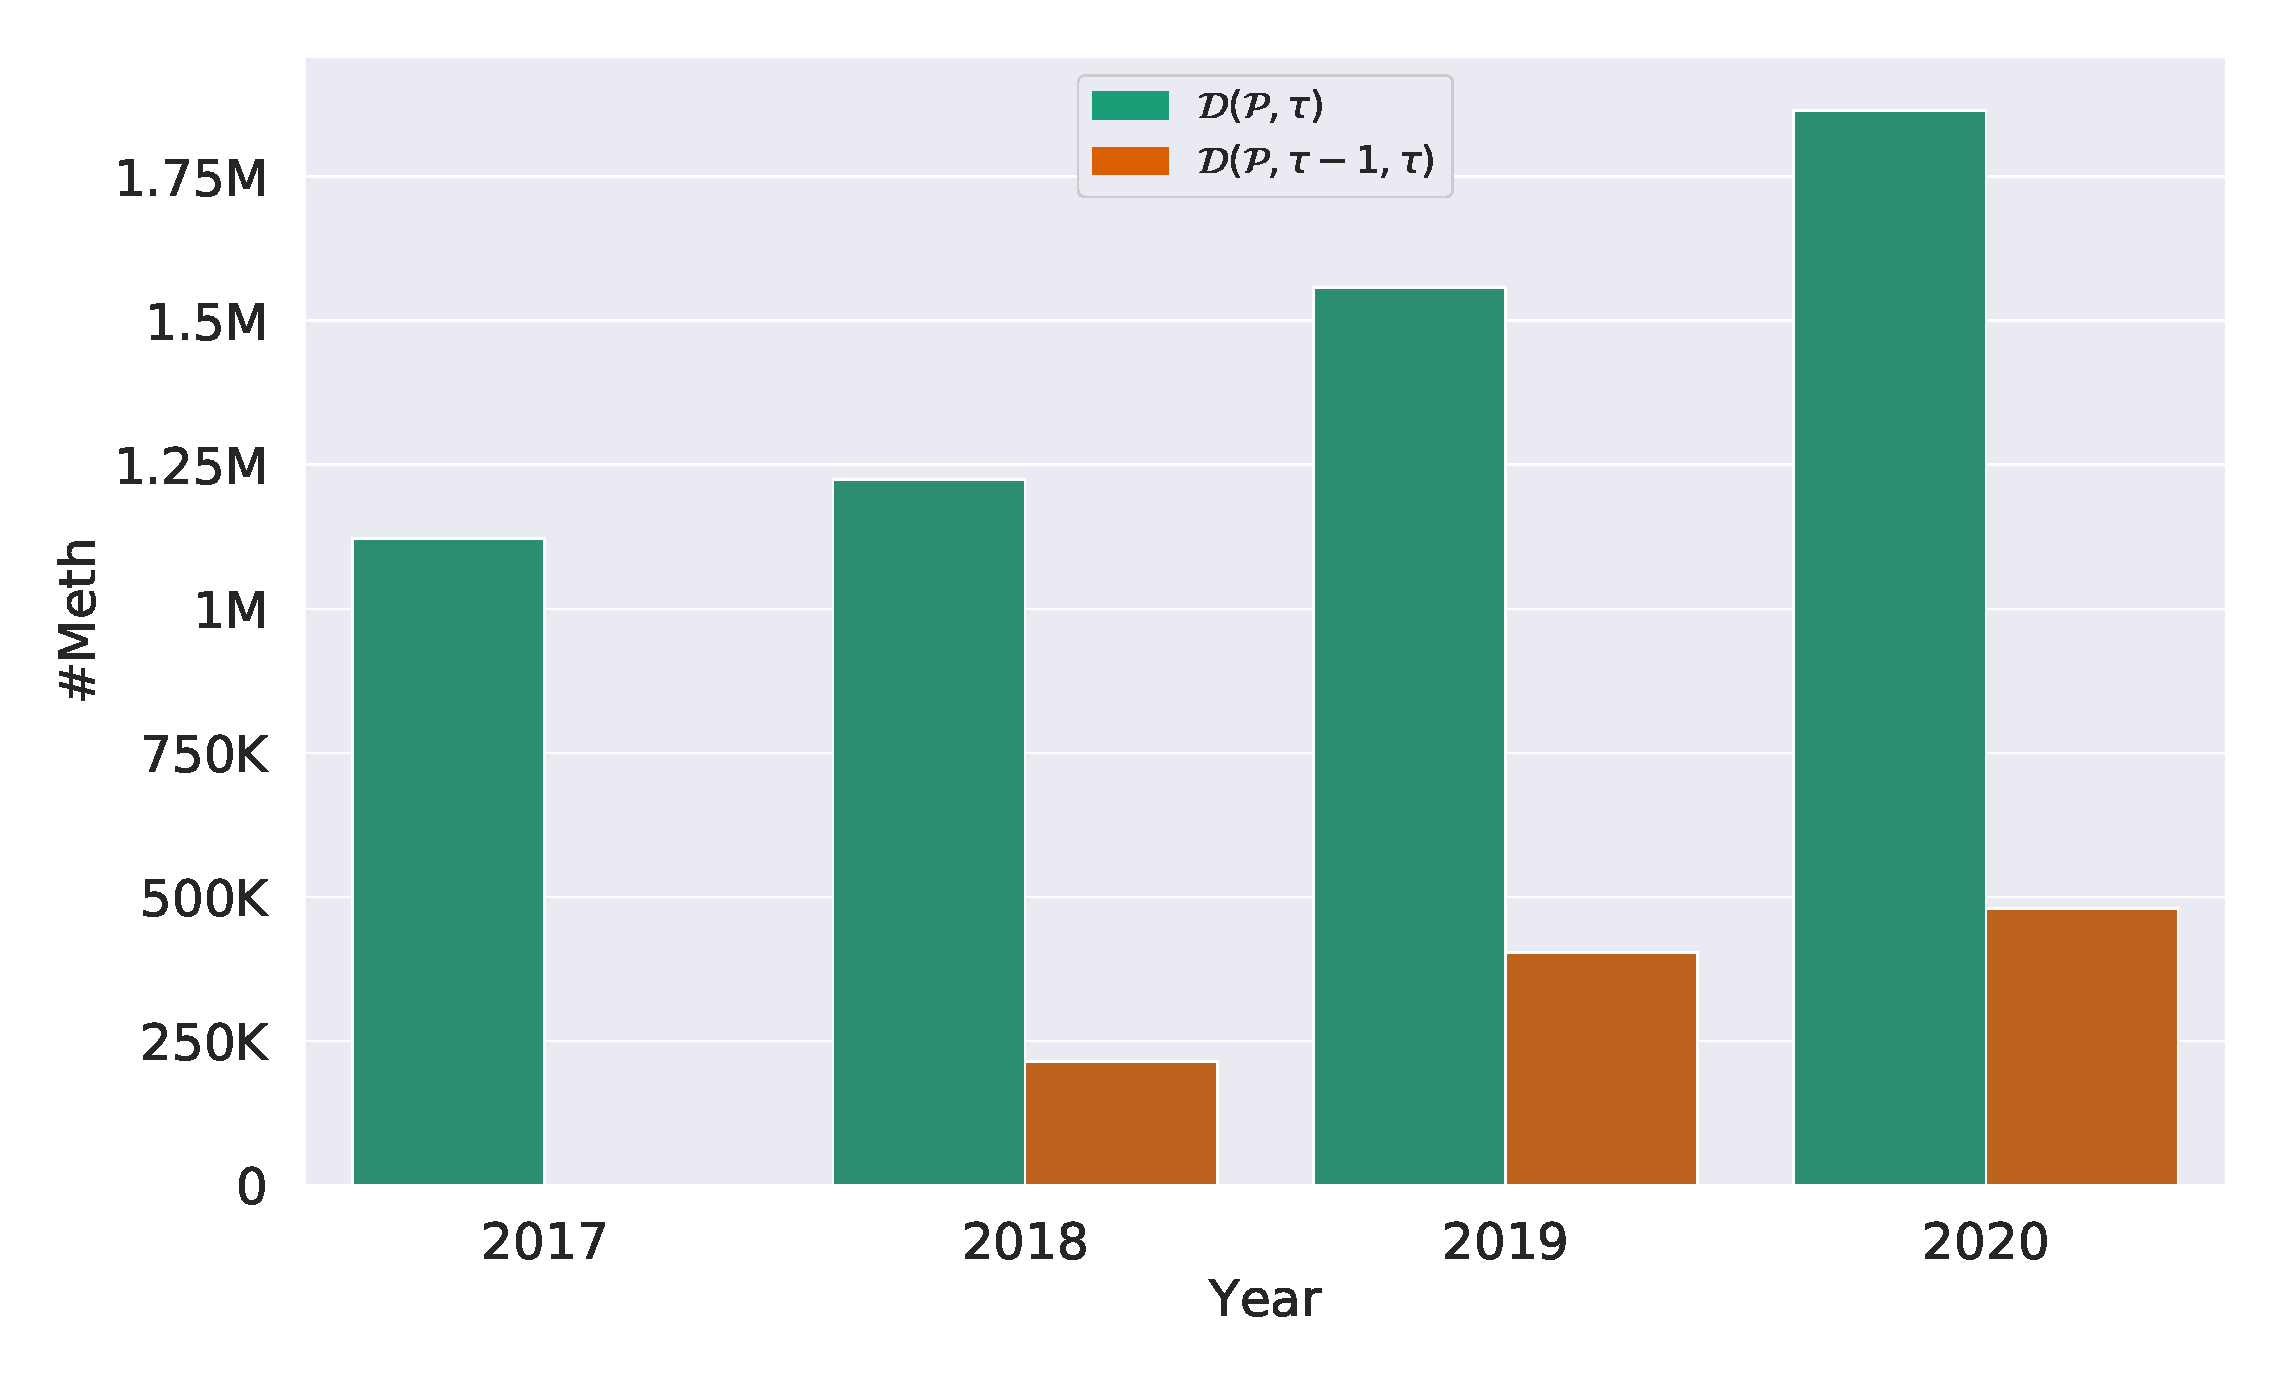
\includegraphics[width=.9\columnwidth]{figs/num-data-evolution.eps}
  \caption{Number of methods on each revision and new to each revision. \label{fig:num-data-evolution}}
\end{figure}

Figure~\ref{fig:num-data-evolution} shows the bar plots of the number
of methods on each revision of the \dataset, as well as the number of
methods new to each revision of the \dataset.  Figure~\ref{X} shows
the bar plots of the average length of methods, comments, and names on
each revision of the \dataset.
